% Diagram: Causal Mask
\begin{figure}[htbp]
\centering
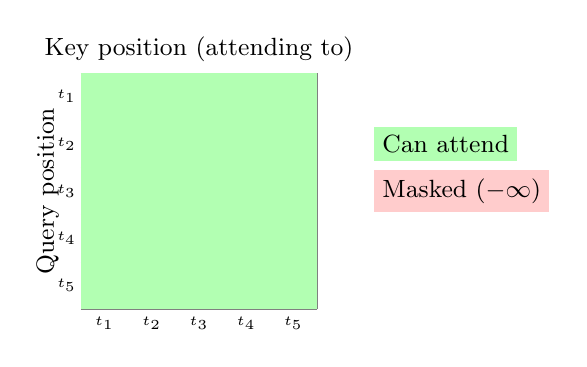
\begin{tikzpicture}[scale=0.6]
% Grid
\draw[step=1cm, gray, very thin] (0,0) grid (5,5);

% Colored cells (lower triangle = can attend)
\foreach \x in {0,...,4} {
    \foreach \y in {0,...,4} {
        \pgfmathtruncatemacro{\sum}{\x + \y}
        \ifnum \y < 5
            \ifnum \x > \y
                \fill[green!30] (\x, 4-\y) rectangle (\x+1, 5-\y);
            \else
                \fill[red!20] (\x, 4-\y) rectangle (\x+1, 5-\y);
            \fi
        \fi
    }
}

% Fix the diagonal and below
\fill[green!30] (0,4) rectangle (1,5);
\fill[green!30] (0,3) rectangle (1,4);
\fill[green!30] (1,3) rectangle (2,4);
\fill[green!30] (0,2) rectangle (1,3);
\fill[green!30] (1,2) rectangle (2,3);
\fill[green!30] (2,2) rectangle (3,3);
\fill[green!30] (0,1) rectangle (1,2);
\fill[green!30] (1,1) rectangle (2,2);
\fill[green!30] (2,1) rectangle (3,2);
\fill[green!30] (3,1) rectangle (4,2);
\fill[green!30] (0,0) rectangle (1,1);
\fill[green!30] (1,0) rectangle (2,1);
\fill[green!30] (2,0) rectangle (3,1);
\fill[green!30] (3,0) rectangle (4,1);
\fill[green!30] (4,0) rectangle (5,1);

% Labels
\node at (2.5, 5.5) {\small Key position (attending to)};
\node[rotate=90] at (-0.7, 2.5) {\small Query position};

% Token labels
\foreach \i in {1,...,5} {
    \node at (\i-0.5, -0.3) {\tiny $t_{\i}$};
    \node at (-0.3, 5.5-\i) {\tiny $t_{\i}$};
}

% Legend
\node[right] at (6, 3.5) {\small \colorbox{green!30}{Can attend}};
\node[right] at (6, 2.5) {\small \colorbox{red!20}{Masked ($-\infty$)}};

\end{tikzpicture}
\caption{Causal attention mask: each token (row) can only attend to itself and earlier tokens (columns).}
\label{fig:causal-mask}
\end{figure}
